\documentclass[RNAAS]{aastex631}

% Numbers are \input from the pipeline-generated macros -- none typed by hand.
% Auto-generated by jansky_research.oamspin.write_paper_macros -- do not edit.
\newcommand{\oamspinSource}{real EHT 2017 data + simulations on its coverage}
\newcommand{\oamspinRealRingRadius}{19.97}
\newcommand{\oamspinRealDz}{545526}
\newcommand{\oamspinSynFfQ}{2.31}
\newcommand{\oamspinSynNoneN}{800}
\newcommand{\oamspinSynNoneLoFid}{0.14}
\newcommand{\oamspinSynNoneHiFid}{6.11}
\newcommand{\oamspinSynNoneLoPone}{0.67}
\newcommand{\oamspinSynNoneHiPone}{1.69}
\newcommand{\oamspinSynNoneMedPone}{1.0}
\newcommand{\oamspinSynNoneExceedPone}{5.1}
\newcommand{\oamspinSynCalN}{120}
\newcommand{\oamspinSynCalLoPone}{0.26}
\newcommand{\oamspinSynCalHiPone}{4.65}
\newcommand{\oamspinRealROneALo}{2.02}
\newcommand{\oamspinRealROneAHi}{1.61}
\newcommand{\oamspinRealROneBLo}{0.94}
\newcommand{\oamspinRealROneBHi}{0.21}
\newcommand{\oamspinRealCombAPone}{0.75}
\newcommand{\oamspinRealCombBPone}{0.82}
\newcommand{\oamspinSynPzeroSymTrue}{1.86}
\newcommand{\oamspinSynPzeroSymRec}{1.0}
\newcommand{\oamspinSynPzeroCresTrue}{99}
\newcommand{\oamspinSynPzeroCresRec}{1.05}


\newcommand{\code}[1]{\texttt{#1}}

\begin{document}

\title{No Separation of Spin from Imaging Noise by the Twisted-Light Estimator for M87*}

\author[0009-0008-3289-4447]{Joseph Barbere}
\affiliation{Independent researcher}

\begin{abstract}
\citet{tamburini2020} derived a spin $a=0.90\pm0.05$ for M87* from an asymmetry $q$ between the
$m=\pm1$ orbital-angular-momentum components of a phase reconstructed from two EHT images taken a
day apart. We applied the published estimator to the public 2017 data and to
\oamspinSynNoneN\ simulated observations of a non-spinning ring on the same baselines. Where $q$
is defined, the simulations give a 95\% range of \oamspinSynNoneLoPone--\oamspinSynNoneHiPone,
which contains the published 1.393, and the real day pairs give \oamspinRealCombAPone\ and
\oamspinRealCombBPone. The reconstruction also cannot recover a phase vortex placed on a symmetric
ring. In these data the estimator does not separate spin from imaging noise.
\end{abstract}

\section{Method}
\label{sec:method}
The estimator of \citet{tamburini2020} recovers a phase $P$ from two intensity images with the
transport-of-intensity equation, $\partial I/\partial z=-(2\pi)^{-1}\nabla\cdot(I\nabla P)$
(their supplementary Eq.~11a), treating the Earth's motion between observing days as the
displacement $z$. It then Fourier analyses $\sqrt{I}\,e^{iP}$ in azimuth around the ring and
takes $q$ as the ratio of the $m=+1$ and $m=-1$ amplitudes. Their two day pairs gave $q=1.417$
and 1.369, mean 1.393, converted to spin through ray-traced rings at an inclination of
$17^\circ$ (their Table~1). Because the brightness is real, its own $m=\pm1$ amplitudes are equal,
so any $q\neq1$ comes from $P$ alone.

We solved the equation by the Fourier method of \citet{teague1983}, centred the analysis annulus
on the ring, and imaged each day of the released calibrated data \citep{ehtdata} with the EHT's
own \code{eht-imaging} pipeline \citep{eht4,chael2016,chael2018}. The paper states no units for
$x$ or $z$. With $x$ measured at M87* and $z$ equal to the Earth's line-of-sight motion in one day
(\oamspinRealDz~km), the recovered phase is of order $10^{16}$~rad and $q$ is meaningless, so we
scaled $z$ over eleven decades and report the range where the phase is of order one radian
(shaded in Figure~\ref{fig:q}).

\section{Tests}
\label{sec:tests}
The null model is a crescent with the radius (\oamspinRealRingRadius~$\mu$as) and brightness
asymmetry of our day-095 image, with no phase structure and no spin. It was observed on the exact
baselines and times of each real day pair with thermal noise, 10\% station gains, random station
phases and the non-closing errors of \citet{eht3}, and imaged with the same pipeline,
\oamspinSynNoneN\ times. Where the phase is near one radian the null gives a median $q$ of
\oamspinSynNoneMedPone\ and a 95\% range of \oamspinSynNoneLoPone--\oamspinSynNoneHiPone;
\oamspinSynNoneExceedPone\% of realisations exceed 1.393. Without station gains
(\oamspinSynCalN\ realisations) the range widens to \oamspinSynCalLoPone--\oamspinSynCalHiPone.
A noiseless crescent observed on two days of real coverage already gives $q=\oamspinSynFfQ$ at the
nominal scaling. The two bands of each 2017 day were recorded simultaneously, yet at the nominal
scaling they give $q=\oamspinRealROneALo$ and \oamspinRealROneAHi\ for days 95--96 and
\oamspinRealROneBLo\ and \oamspinRealROneBHi\ for days 100--101. Imaged with both bands together,
the day pairs give \oamspinRealCombAPone\ and \oamspinRealCombBPone\ where the phase is near one
radian.

A further test needs no data. For a phase vortex $P=\alpha\phi$ the change of intensity between
the two planes is proportional to $\partial I/\partial\phi$, so on an azimuthally symmetric ring a
vortex leaves both images identical. A vortex with $q=\oamspinSynPzeroSymTrue$ on a symmetric ring
is recovered as $q=\oamspinSynPzeroSymRec$, and an $\ell=1$ vortex ($q=\oamspinSynPzeroCresTrue$) on
the M87* crescent as $q=\oamspinSynPzeroCresRec$. The reconstruction keeps only the curl-free
part of $I\nabla P$, which discards the circulation that carries the orbital angular momentum.

\section{Conclusion}
\label{sec:conclusion}
On the 2017 baselines the published $q$ lies within the spread produced by imaging a
non-spinning ring, the real day pairs do not reproduce it, and the two-image reconstruction cannot
carry the signal it is meant to measure. These results apply to the method as published and as
implemented here; the authors' code and input images are not public. They do not bear on the spin
of M87*, for which other constraints exist \citep{eht1}.

\begin{figure}[ht]
\centering
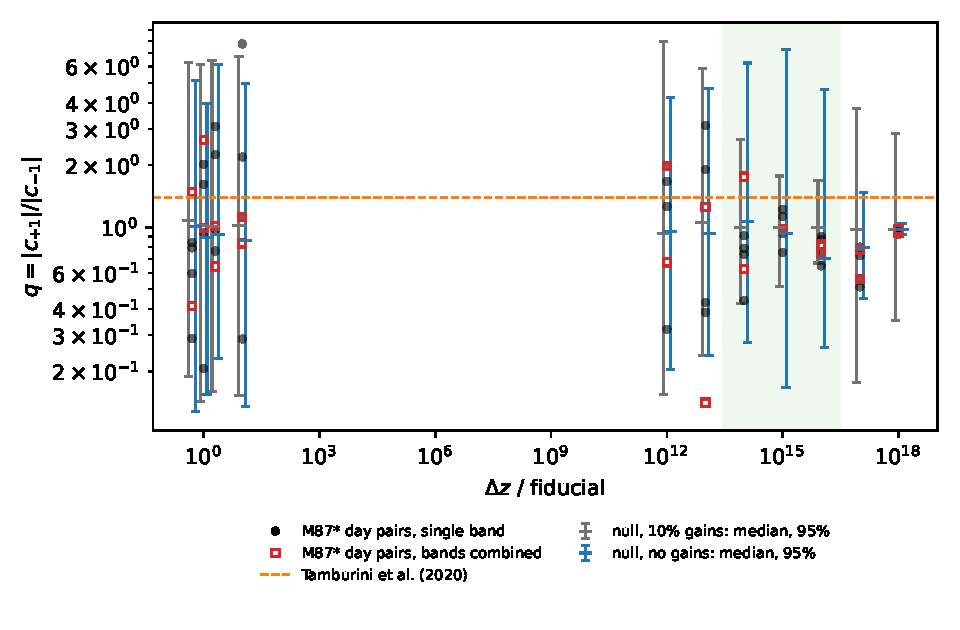
\includegraphics[width=\linewidth]{figures/oamspin_q.pdf}
\caption{The asymmetry $q$ against the assumed displacement $\Delta z$, relative to the Earth's
one-day motion. Bars give the median and 95\% range of the non-spinning null with and without
station gains; circles and squares are the 2017 day pairs imaged by band and with both bands
together; the dashed line is the published value. The shaded band marks where the recovered phase
is of order one radian.}
\label{fig:q}
\end{figure}

\software{\code{jansky-research} \citep{janskyresearch}, \code{jansky} \citep{jansky},
\code{eht-imaging} \citep{chael2016,chael2018}, NumPy, SciPy, Astropy, Matplotlib. Analysis assisted
by Claude \citep{anthropicclaude}. The estimator and its controls are covered by an offline test
suite; the imaging and simulation drivers are not unit-tested.}

\bibliography{refs}
\bibliographystyle{aasjournal}

\end{document}
